% ----------------------------------------------------------------------
%
%                            TFMTesis.tex
%
%----------------------------------------------------------------------
%
% Este fichero contiene el "documento maestro" del documento. Lo único
% que hace es configurar el entorno LaTeX e incluir los ficheros .tex
% que contienen cada sección.
%
%----------------------------------------------------------------------
%
% Los ficheros necesarios para este documento son:
%
%       TeXiS/* : ficheros de la plantilla TeXiS.
%       Cascaras/* : ficheros con las partes del documento que no
%          son capítulos ni apéndices (portada, agradecimientos, etc.)
%       Capitulos/*.tex : capítulos de la tesis
%       Apendices/*.tex: apéndices de la tesis
%       constantes.tex: constantes LaTeX
%       config.tex : configuración de la "compilación" del documento
%       guionado.tex : palabras con guiones
%
% Para la bibliografía, además, se necesitan:
%
%       *.bib : ficheros con la información de las referencias
%
% ---------------------------------------------------------------------

\documentclass[12pt,a4paper,twoside]{book}

%
% Definimos  el   comando  \compilaCapitulo,  que   luego  se  utiliza
% (opcionalmente) en config.tex. Quedaría  mejor si también se definiera
% en  ese fichero,  pero por  el modo  en el  que funciona  eso  no es
% posible. Puedes consultar la documentación de ese fichero para tener
% más  información. Definimos también  \compilaApendice, que  tiene el
% mismo  cometido, pero  que se  utiliza para  compilar  únicamente un
% apéndice.
%
%
% Si  queremos   compilar  solo   una  parte  del   documento  podemos
% especificar mediante  \includeonly{...} qué ficheros  son los únicos
% que queremos  que se incluyan.  Esto  es útil por  ejemplo para sólo
% compilar un capítulo.
%
% El problema es que todos aquellos  ficheros que NO estén en la lista
% NO   se  incluirán...  y   eso  también   afecta  a   ficheros  de
% la plantilla...
%
% Total,  que definimos  una constante  con los  ficheros  que siempre
% vamos a querer compilar  (aquellos relacionados con configuración) y
% luego definimos \compilaCapitulo.
\newcommand{\ficherosBasicosTeXiS}{%
TeXiS/TeXiS_pream,TeXiS/TeXiS_cab,TeXiS/TeXiS_bib,TeXiS/TeXiS_cover%
}
\newcommand{\ficherosBasicosTexto}{%
constantes,guionado,Cascaras/bibliografia,config%
}
\newcommand{\compilaCapitulo}[1]{%
\includeonly{\ficherosBasicosTeXiS,\ficherosBasicosTexto,Capitulos/#1}%
}

\newcommand{\compilaApendice}[1]{%
\includeonly{\ficherosBasicosTeXiS,\ficherosBasicosTexto,Apendices/#1}%
}

%- - - - - - - - - - - - - - - - - - - - - - - - - - - - - - - - - - -
%            Preámbulo del documento. Configuraciones varias
%- - - - - - - - - - - - - - - - - - - - - - - - - - - - - - - - - - -

% Define  el  tipo  de  compilación que  estamos  haciendo.   Contiene
% definiciones  de  constantes que  cambian  el  comportamiento de  la
% compilación. Debe incluirse antes del paquete TeXiS/TeXiS.sty
%---------------------------------------------------------------------
%
%                          config.tex
%
%---------------------------------------------------------------------
%
% Contiene la  definición de constantes  que determinan el modo  en el
% que se compilará el documento.
%
%---------------------------------------------------------------------
%
% En concreto, podemos  indicar si queremos "modo release",  en el que
% no  aparecerán  los  comentarios  (creados  mediante  \com{Texto}  o
% \comp{Texto}) ni los "por  hacer" (creados mediante \todo{Texto}), y
% sí aparecerán los índices. El modo "debug" (o mejor dicho en modo no
% "release" muestra los índices  (construirlos lleva tiempo y son poco
% útiles  salvo  para   la  versión  final),  pero  sí   el  resto  de
% anotaciones.
%
% Si se compila con LaTeX (no  con pdflatex) en modo Debug, también se
% muestran en una esquina de cada página las entradas (en el índice de
% palabras) que referencian  a dicha página (consulta TeXiS_pream.tex,
% en la parte referente a show).
%
% El soporte para  el índice de palabras en  TeXiS es embrionario, por
% lo  que no  asumas que  esto funcionará  correctamente.  Consulta la
% documentación al respecto en TeXiS_pream.tex.
%
%
% También  aquí configuramos  si queremos  o  no que  se incluyan  los
% acrónimos  en el  documento final  en la  versión release.  Para eso
% define (o no) la constante \acronimosEnRelease.
%
% Utilizando \compilaCapitulo{nombre}  podemos también especificar qué
% capítulo(s) queremos que se compilen. Si no se pone nada, se compila
% el documento  completo.  Si se pone, por  ejemplo, 01Introduccion se
% compilará únicamente el fichero Capitulos/01Introduccion.tex
%
% Para compilar varios  capítulos, se separan sus nombres  con comas y
% no se ponen espacios de separación.
%
% En realidad  la macro \compilaCapitulo  está definida en  el fichero
% principal tesis.tex.
%
%---------------------------------------------------------------------


% Comentar la línea si no se compila en modo release.
% TeXiS hará el resto.
% ¡¡¡Si cambias esto, haz un make clean antes de recompilar!!!
%\def\release{1}


% Descomentar la linea si se quieren incluir los
% acrónimos en modo release (en modo debug
% no se incluirán nunca).
% ¡¡¡Si cambias esto, haz un make clean antes de recompilar!!!
\def\acronimosEnRelease{1}


% Descomentar la línea para establecer el capítulo que queremos
% compilar

% \compilaCapitulo{01Introduccion}
% \compilaCapitulo{02EstructuraYGeneracion}
% \compilaCapitulo{03Edicion}
% \compilaCapitulo{04Imagenes}
% \compilaCapitulo{05Bibliografia}
% \compilaCapitulo{06Makefile}

% \compilaApendice{01AsiSeHizo}

% Variable local para emacs, para  que encuentre el fichero maestro de
% compilación y funcionen mejor algunas teclas rápidas de AucTeX
%%%
%%% Local Variables:
%%% mode: latex
%%% TeX-master: "./Tesis.tex"
%%% End:


% Paquete de la plantilla
\usepackage{TeXiS/TeXiS}

% Incluimos el fichero con comandos de constantes
%---------------------------------------------------------------------
%
%                          constantes.tex
%
%---------------------------------------------------------------------
%
% Fichero que  declara nuevos comandos LaTeX  sencillos realizados por
% comodidad en la escritura de determinadas palabras
%
%---------------------------------------------------------------------

%%%%%%%%%%%%%%%%%%%%%%%%%%%%%%%%%%%%%%%%%%%%%%%%%%%%%%%%%%%%%%%%%%%%%%
% Comando: 
%
%       \titulo
%
% Resultado: 
%
% Escribe el título del documento.
%%%%%%%%%%%%%%%%%%%%%%%%%%%%%%%%%%%%%%%%%%%%%%%%%%%%%%%%%%%%%%%%%%%%%%
\def\titulo{\textsc{TeXiS}: Una plantilla de \LaTeX\
  para Tesis y otros documentos}

%%%%%%%%%%%%%%%%%%%%%%%%%%%%%%%%%%%%%%%%%%%%%%%%%%%%%%%%%%%%%%%%%%%%%%
% Comando: 
%
%       \autor
%
% Resultado: 
%
% Escribe el autor del documento.
%%%%%%%%%%%%%%%%%%%%%%%%%%%%%%%%%%%%%%%%%%%%%%%%%%%%%%%%%%%%%%%%%%%%%%
\def\autor{Marco Antonio y Pedro Pablo G\'omez Mart\'in}

% Variable local para emacs, para  que encuentre el fichero maestro de
% compilación y funcionen mejor algunas teclas rápidas de AucTeX

%%%
%%% Local Variables:
%%% mode: latex
%%% TeX-master: "tesis.tex"
%%% End:


% Sacamos en el log de la compilación el copyright
%\typeout{Copyright Marco Antonio and Pedro Pablo Gomez Martin}

%
% "Metadatos" para el PDF
%
\ifpdf\hypersetup{%
    pdftitle = {\titulo},
    pdfsubject = {Plantilla de Tesis},
    pdfkeywords = {Plantilla, LaTeX, tesis, trabajo de
      investigación, trabajo de Master},
    pdfauthor = {\textcopyright\ \autor},
    pdfcreator = {\LaTeX\ con el paquete \flqq hyperref\frqq},
    pdfproducer = {pdfeTeX-0.\the\pdftexversion\pdftexrevision},
    }
    \pdfinfo{/CreationDate (\today)}
\fi


%- - - - - - - - - - - - - - - - - - - - - - - - - - - - - - - - - - -
%                        Documento
%- - - - - - - - - - - - - - - - - - - - - - - - - - - - - - - - - - -
\begin{document}

% Incluimos el  fichero de definición de guionado  de algunas palabras
% que LaTeX no ha dividido como debería
%----------------------------------------------------------------
%
%                          guionado.tex
%
%----------------------------------------------------------------
%
% Fichero con algunas divisiones de palabras que LaTeX no
% hace correctamente si no se le da alguna ayuda.
%
%----------------------------------------------------------------

\hyphenation{
% a
abs-trac-to
abs-trac-tos
abs-trac-ta
abs-trac-tas
ac-tua-do-res
a-gra-de-ci-mien-tos
ana-li-za-dor
an-te-rio-res
an-te-rior-men-te
apa-rien-cia
a-pro-pia-do
a-pro-pia-dos
a-pro-pia-da
a-pro-pia-das
a-pro-ve-cha-mien-to
a-que-llo
a-que-llos
a-que-lla
a-que-llas
a-sig-na-tu-ra
a-sig-na-tu-ras
a-so-cia-da
a-so-cia-das
a-so-cia-do
a-so-cia-dos
au-to-ma-ti-za-do
% b
batch
bi-blio-gra-fía
bi-blio-grá-fi-cas
bien
bo-rra-dor
boo-l-ean-expr
% c
ca-be-ce-ra
call-me-thod-ins-truc-tion
cas-te-lla-no
cir-cuns-tan-cia
cir-cuns-tan-cias
co-he-ren-te
co-he-ren-tes
co-he-ren-cia
co-li-bri
co-men-ta-rio
co-mer-cia-les
co-no-ci-mien-to
cons-cien-te
con-si-de-ra-ba
con-si-de-ra-mos
con-si-de-rar-se
cons-tan-te
cons-trucción
cons-tru-ye
cons-tru-ir-se
con-tro-le
co-rrec-ta-men-te
co-rres-pon-den
co-rres-pon-dien-te
co-rres-pon-dien-tes
co-ti-dia-na
co-ti-dia-no
crean
cris-ta-li-zan
cu-rri-cu-la
cu-rri-cu-lum
cu-rri-cu-lar
cu-rri-cu-la-res
% d
de-di-ca-do
de-di-ca-dos
de-di-ca-da
de-di-ca-das
de-rro-te-ro
de-rro-te-ros
de-sa-rro-llo
de-sa-rro-llos
de-sa-rro-lla-do
de-sa-rro-lla-dos
de-sa-rro-lla-da
de-sa-rro-lla-das
de-sa-rro-lla-dor
de-sa-rro-llar
des-cri-bi-re-mos
des-crip-ción
des-crip-cio-nes
des-cri-to
des-pués
de-ta-lla-do
de-ta-lla-dos
de-ta-lla-da
de-ta-lla-das
di-a-gra-ma
di-a-gra-mas
di-se-ños
dis-po-ner
dis-po-ni-bi-li-dad
do-cu-men-ta-da
do-cu-men-to
do-cu-men-tos
% e
edi-ta-do
e-du-ca-ti-vo
e-du-ca-ti-vos
e-du-ca-ti-va
e-du-ca-ti-vas
e-la-bo-ra-do
e-la-bo-ra-dos
e-la-bo-ra-da
e-la-bo-ra-das
es-co-llo
es-co-llos
es-tu-dia-do
es-tu-dia-dos
es-tu-dia-da
es-tu-dia-das
es-tu-dian-te
e-va-lua-cio-nes
e-va-lua-do-res
exis-ten-tes
exhaus-ti-va
ex-pe-rien-cia
ex-pe-rien-cias
% f
for-ma-li-za-do
% g
ge-ne-ra-ción
ge-ne-ra-dor
ge-ne-ra-do-res
ge-ne-ran
% h
he-rra-mien-ta
he-rra-mien-tas
% i
i-dio-ma
i-dio-mas
im-pres-cin-di-ble
im-pres-cin-di-bles
in-de-xa-do
in-de-xa-dos
in-de-xa-da
in-de-xa-das
in-di-vi-dual
in-fe-ren-cia
in-fe-ren-cias
in-for-ma-ti-ca
in-gre-dien-te
in-gre-dien-tes
in-me-dia-ta-men-te
ins-ta-la-do
ins-tan-cias
% j
% k
% l
len-gua-je
li-be-ra-to-rio
li-be-ra-to-rios
li-be-ra-to-ria
li-be-ra-to-rias
li-mi-ta-do
li-te-ra-rio
li-te-ra-rios
li-te-ra-ria
li-te-ra-rias
lo-tes
% m
ma-ne-ra
ma-nual
mas-que-ra-de
ma-yor
me-mo-ria
mi-nis-te-rio
mi-nis-te-rios
mo-de-lo
mo-de-los
mo-de-la-do
mo-du-la-ri-dad
mo-vi-mien-to
% n
na-tu-ral
ni-vel
nues-tro
% o
obs-tan-te
o-rien-ta-do
o-rien-ta-dos
o-rien-ta-da
o-rien-ta-das
% p
pa-ra-le-lo
pa-ra-le-la
par-ti-cu-lar
par-ti-cu-lar-men-te
pe-da-gó-gi-ca
pe-da-gó-gi-cas
pe-da-gó-gi-co
pe-da-gó-gi-cos
pe-rio-di-ci-dad
per-so-na-je
plan-te-a-mien-to
plan-te-a-mien-tos
po-si-ción
pre-fe-ren-cia
pre-fe-ren-cias
pres-cin-di-ble
pres-cin-di-bles
pri-me-ra
pro-ble-ma
pro-ble-mas
pró-xi-mo
pu-bli-ca-cio-nes
pu-bli-ca-do
% q
% r
rá-pi-da
rá-pi-do
ra-zo-na-mien-to
ra-zo-na-mien-tos
re-a-li-zan-do
re-fe-ren-cia
re-fe-ren-cias
re-fe-ren-cia-da
re-fe-ren-cian
re-le-van-tes
re-pre-sen-ta-do
re-pre-sen-ta-dos
re-pre-sen-ta-da
re-pre-sen-ta-das
re-pre-sen-tar-lo
re-qui-si-to
re-qui-si-tos
res-pon-der
res-pon-sa-ble
% s
se-pa-ra-do
si-guien-do
si-guien-te
si-guien-tes
si-guie-ron
si-mi-lar
si-mi-la-res
si-tua-ción
% t
tem-pe-ra-ments
te-ner
trans-fe-ren-cia
trans-fe-ren-cias
% u
u-sua-rio
Unreal-Ed
% v
va-lor
va-lo-res
va-rian-te
ver-da-de-ro
ver-da-de-ros
ver-da-de-ra
ver-da-de-ras
ver-da-de-ra-men-te
ve-ri-fi-ca
% w
% x
% y
% z
}
% Variable local para emacs, para que encuentre el fichero
% maestro de compilación
%%%
%%% Local Variables:
%%% mode: latex
%%% TeX-master: "./Tesis.tex"
%%% End:


% Marcamos  el inicio  del  documento para  la  numeración de  páginas
% (usando números romanos para esta primera fase).
\frontmatter
\pagestyle{empty}

%---------------------------------------------------------------------
%
%                          configCover.tex
%
%---------------------------------------------------------------------
%
% cover.tex
% Copyright 2009 Marco Antonio Gomez-Martin, Pedro Pablo Gomez-Martin
%
% This file belongs to the TeXiS manual, a LaTeX template for writting
% Thesis and other documents. The complete last TeXiS package can
% be obtained from http://gaia.fdi.ucm.es/projects/texis/
%
% Although the TeXiS template itself is distributed under the 
% conditions of the LaTeX Project Public License
% (http://www.latex-project.org/lppl.txt), the manual content
% uses the CC-BY-SA license that stays that you are free:
%
%    - to share & to copy, distribute and transmit the work
%    - to remix and to adapt the work
%
% under the following conditions:
%
%    - Attribution: you must attribute the work in the manner
%      specified by the author or licensor (but not in any way that
%      suggests that they endorse you or your use of the work).
%    - Share Alike: if you alter, transform, or build upon this
%      work, you may distribute the resulting work only under the
%      same, similar or a compatible license.
%
% The complete license is available in
% http://creativecommons.org/licenses/by-sa/3.0/legalcode
%
%---------------------------------------------------------------------
%
% Fichero que contiene la configuración de la portada y de la 
% primera hoja del documento.
%
%---------------------------------------------------------------------


% Pueden configurarse todos los elementos del contenido de la portada
% utilizando comandos.

%%%%%%%%%%%%%%%%%%%%%%%%%%%%%%%%%%%%%%%%%%%%%%%%%%%%%%%%%%%%%%%%%%%%%%
% Título del documento:
% \tituloPortada{titulo}
% Nota:
% Si no se define se utiliza el del \titulo. Este comando permite
% cambiar el título de forma que se especifiquen dónde se quieren
% los retornos de carro cuando se utilizan fuentes grandes.
%%%%%%%%%%%%%%%%%%%%%%%%%%%%%%%%%%%%%%%%%%%%%%%%%%%%%%%%%%%%%%%%%%%%%%
\tituloPortada{%
%Título en español \textcolor{red}{(definido en Cascaras$\backslash$cover.tex)}
Framework de comportamientos de enemigos para videojuegos 2D
}


%%%%%%%%%%%%%%%%%%%%%%%%%%%%%%%%%%%%%%%%%%%%%%%%%%%%%%%%%%%%%%%%%%%%%%
% Título del documento en inglés:
% \tituloPortadaEng{titulo}
% Nota:
% Si no se define se utiliza el del \titulo. Este comando permite
% cambiar el título de forma que se especifiquen dónde se quieren
% los retornos de carro cuando se utilizan fuentes grandes.
%%%%%%%%%%%%%%%%%%%%%%%%%%%%%%%%%%%%%%%%%%%%%%%%%%%%%%%%%%%%%%%%%%%%%%
\tituloPortadaEng{%
%Title in English \textcolor{red}{(defined in Cascaras$\backslash$cover.tex)}
An enemy behaviour framework for 2D videogames
}

%%%%%%%%%%%%%%%%%%%%%%%%%%%%%%%%%%%%%%%%%%%%%%%%%%%%%%%%%%%%%%%%%%%%%%
% Autor del documento:
% \autorPortada{Nombre}
% Se utiliza en la portada y en el valor por defecto del
% primer subtítulo de la segunda portada.
%%%%%%%%%%%%%%%%%%%%%%%%%%%%%%%%%%%%%%%%%%%%%%%%%%%%%%%%%%%%%%%%%%%%%%
\autorPortada{Francisco Miguel Galván Muñoz \\Cristina Mora Velasco}
%%%%%%%%%%%%%%%%%%%%%%%%%%%%%%%%%%%%%%%%%%%%%%%%%%%%%%%%%%%%%%%%%%%%%%
% Fecha de publicación:
% \fechaPublicacion{Fecha}
% Puede ser vacío. Aparece en la última línea de ambas portadas
%%%%%%%%%%%%%%%%%%%%%%%%%%%%%%%%%%%%%%%%%%%%%%%%%%%%%%%%%%%%%%%%%%%%%%
% Descomentar para que ponga siempre la fecha actual
%\fechaPublicacion{\today}
\fechaPublicacion{13 de Junio de 2025}

%%%%%%%%%%%%%%%%%%%%%%%%%%%%%%%%%%%%%%%%%%%%%%%%%%%%%%%%%%%%%%%%%%%%%%
% Imagen de la portada (y escala)
% \imagenPortada{Fichero}
% \escalaImagenPortada{Numero}
% Si no se especifica, se utiliza la imagen TODO.pdf
%%%%%%%%%%%%%%%%%%%%%%%%%%%%%%%%%%%%%%%%%%%%%%%%%%%%%%%%%%%%%%%%%%%%%%
% imagen en blanco y negro
%\imagenPortada{Imagenes/Vectorial/escudoUCM}
%imagen en color
\imagenPortada{Imagenes/Bitmap/escudoUCMcolor}
\escalaImagenPortada{.2}

%%%%%%%%%%%%%%%%%%%%%%%%%%%%%%%%%%%%%%%%%%%%%%%%%%%%%%%%%%%%%%%%%%%%%%
% Tipo de documento.
% \tipoDocumento{Tipo}
% Para el texto justo debajo del escudo.
% Si no se indica, se utiliza "TESIS\ DOCTORAL".
%%%%%%%%%%%%%%%%%%%%%%%%%%%%%%%%%%%%%%%%%%%%%%%%%%%%%%%%%%%%%%%%%%%%%%
\tipoDocumento{Trabajo de Fin de Grado}

%%%%%%%%%%%%%%%%%%%%%%%%%%%%%%%%%%%%%%%%%%%%%%%%%%%%%%%%%%%%%%%%%%%%%%
% Institución/departamento asociado al documento.
% \institucion{Nombre}
% Puede tener varias líneas. Se utiliza en las dos portadas.
% Si no se indica aparecerá vacío.
%%%%%%%%%%%%%%%%%%%%%%%%%%%%%%%%%%%%%%%%%%%%%%%%%%%%%%%%%%%%%%%%%%%%%%
\institucion{%
Grado en {Desarrollo de Videojuegos}\\[0.2em]
Facultad de Informática\\[0.2em]
Universidad Complutense de Madrid
}

%%%%%%%%%%%%%%%%%%%%%%%%%%%%%%%%%%%%%%%%%%%%%%%%%%%%%%%%%%%%%%%%%%%%%%
% Director del trabajo.
% \directorPortada{Nombre}
% Se utiliza para el valor por defecto del segundo subtítulo, donde
% se indica quién es el director del trabajo.
% Si se fuerza un subtítulo distinto, no hace falta definirlo.
%%%%%%%%%%%%%%%%%%%%%%%%%%%%%%%%%%%%%%%%%%%%%%%%%%%%%%%%%%%%%%%%%%%%%%
\directorPortada{Guillermo Jimenez Díaz}


%%%%%%%%%%%%%%%%%%%%%%%%%%%%%%%%%%%%%%%%%%%%%%%%%%%%%%%%%%%%%%%%%%%%%%
% Colaborador en la dirección del trabajo.
% \colaboradorPortada{Nombre}
% Se utiliza para el valor por defecto del segundo subtítulo, donde
% se indica quién es el colaborador en la dirección del trabajo.
% Si se fuerza un subtítulo distinto, no hace falta definirlo.
%%%%%%%%%%%%%%%%%%%%%%%%%%%%%%%%%%%%%%%%%%%%%%%%%%%%%%%%%%%%%%%%%%%%%%
\colaboradorPortada{{Guillermo Jimenez Díaz}}


%%%%%%%%%%%%%%%%%%%%%%%%%%%%%%%%%%%%%%%%%%%%%%%%%%%%%%%%%%%%%%%%%%%%%%
% Texto del primer subtítulo de la segunda portada.
% \textoPrimerSubtituloPortada{Texto}
% Para configurar el primer "texto libre" de la segunda portada.
% Si no se especifica se indica "Memoria que presenta para optar al
% título de Doctor en Informática" seguido del \autorPortada.
%%%%%%%%%%%%%%%%%%%%%%%%%%%%%%%%%%%%%%%%%%%%%%%%%%%%%%%%%%%%%%%%%%%%%%
\textoPrimerSubtituloPortada{%
\textbf{Trabajo de Fin de Grado en {Desarrollo de Videojuegos}\\ [0.3em]
}

%%%%%%%%%%%%%%%%%%%%%%%%%%%%%%%%%%%%%%%%%%%%%%%%%%%%%%%%%%%%%%%%%%%%%%
% Texto del segundo subtítulo de la segunda portada.
% \textoSegundoSubtituloPortada{Texto}
% Para configurar el segundo "texto libre" de la segunda portada.
% Si no se especifica se indica "Dirigida por el Doctor" seguido
% del \directorPortada.
%%%%%%%%%%%%%%%%%%%%%%%%%%%%%%%%%%%%%%%%%%%%%%%%%%%%%%%%%%%%%%%%%%%%%%
\textoSegundoSubtituloPortada{%
\textbf{Convocatoria: }{Junio} \the\year}%\\[0.2em]
\textbf{Calificación: }\textit{Cristina Mora Velasco: 9.2\\
Francisco Miguel Galván Muñoz: 9.2}
}

%%%%%%%%%%%%%%%%%%%%%%%%%%%%%%%%%%%%%%%%%%%%%%%%%%%%%%%%%%%%%%%%%%%%%%
% \explicacionDobleCara
% Si se utiliza, se aclara que el documento está preparado para la
% impresión a doble cara.
%%%%%%%%%%%%%%%%%%%%%%%%%%%%%%%%%%%%%%%%%%%%%%%%%%%%%%%%%%%%%%%%%%%%%%
%\explicacionDobleCara

%%%%%%%%%%%%%%%%%%%%%%%%%%%%%%%%%%%%%%%%%%%%%%%%%%%%%%%%%%%%%%%%%%%%%%
% \isbn
% Si se utiliza, aparecerá el ISBN detrás de la segunda portada.
%%%%%%%%%%%%%%%%%%%%%%%%%%%%%%%%%%%%%%%%%%%%%%%%%%%%%%%%%%%%%%%%%%%%%%
%\isbn{978-84-692-7109-4}


%%%%%%%%%%%%%%%%%%%%%%%%%%%%%%%%%%%%%%%%%%%%%%%%%%%%%%%%%%%%%%%%%%%%%%
% \copyrightInfo
% Si se utiliza, aparecerá información de los derechos de copyright
% detrás de la segunda portada.
%%%%%%%%%%%%%%%%%%%%%%%%%%%%%%%%%%%%%%%%%%%%%%%%%%%%%%%%%%%%%%%%%%%%%%
%\copyrightInfo{\autor}


%%
%% Creamos las portadas
%%
\makeCover

% Variable local para emacs, para que encuentre el fichero
% maestro de compilación
%%%
%%% Local Variables:
%%% mode: latex
%%% TeX-master: "../Tesis.tex"
%%% End:

%\include{Cascaras/autorizacion}
% +--------------------------------------------------------------------+
% | Dedication Page (Optional)
% +--------------------------------------------------------------------+

\chapter*{Dedicatoria}

% Primera dedicatoria a la derecha
\begin{flushright}
\begin{minipage}[c]{8.5cm}
\flushright{\textit{
A nuestras familias por el apoyo incondicional mostrado en la consecución de este trabajo.\\ 
Y a nuestras gatas por inventar el arte de convertir el dolor de un arañazo en la alegría de un beso.\\
}}
\end{minipage}
\end{flushright}

\vspace{1cm} % Espacio vertical entre las dedicatorias

% Segunda dedicatoria a la izquierda
\begin{flushleft}
\begin{minipage}[c]{8.5cm}
\flushleft{\textit{
Quiero dedicar este trabajo a todos los que me vieron iniciar esta aventura y no pudieron ver su consecución. Sin vosotros no habría llegado hasta aquí.\\
}}
\end{minipage}
\end{flushleft}


% +--------------------------------------------------------------------+
% | Acknowledgements Page (Optional)                                   |
% +--------------------------------------------------------------------+

\chapter*{Agradecimientos}

A Guillermo por ser el mejor tutor de Trabajo de Fin de Grado posible y por habernos dado la oportunidad de complir un sueño al llegar a la consecución de este grado.











\chapter*{Resumen}

\section*{\tituloPortadaVal}

La creación de un videojuego es la combinación homogénea de varias disciplinas para crear una experiencia interactiva. Entre estas disciplinas encontramos arte, sonido, programación y diseño. A la hora de hacer arte, el ser humano siempre se ha ayudado de herramientas fabricadas por él mismo y le ha ayudado a llevar a cabo las tareas de manera más eficaz y precisa.
A la hora de hacer un videojuego de cualquier tipo, el equipo detrás de la obra tiene que dejar clara dos ideas al jugador: el objetivo del juego y los obstáculos a los que se va a tener que enfrentar para alcanzarlo. Haciendo especial hincapié en que en el tipo de juegos analizados en este trabajo, el principal obstáculo serán enemigos. Para que estos supongan un desafío para el jugador deberán contar con una inteligencia artificial acorde al diseño del mismo.\\\\ 

El objetivo de este trabajo es desarrollar una herramienta cuyo propósito sea generar enemigos para videojuegos de plataformas 2D. Para ello se diseñará un catálogo de componentes para Unity que permitirá crear, sin tener conocimientos previos de programación, comportamientos de enemigos. Este catálogo de componentes es el resultado de nuestro trabajo de investigación y posterior abstracción de comportamientos de enemigos en juegos de plataformas 2D. 
\section*{Palabras clave}
   
\noindent Inteligencia Artificial, IA, Unity, Enemigo, Maquinas de Estado, Estado, Sensor

   



\begin{otherlanguage}{english}
\chapter*{Abstract}

\section*{\tituloPortadaEngVal}

An abstract in English, half a page long, including the title in English. Below, a list with no more than 10 keywords.


\section*{Keywords}

\noindent 10 keywords max., separated by commas.




% Si el trabajo se escribe en inglés, comentar esta línea y descomentar
% otra igual que hay justo antes de \end{document}
\end{otherlanguage}

\ifx\generatoc\undefined
\else
%---------------------------------------------------------------------
%
%                          TeXiS_toc.tex
%
%---------------------------------------------------------------------
%
% TeXiS_toc.tex
% Copyright 2009 Marco Antonio Gomez-Martin, Pedro Pablo Gomez-Martin
%
% This file belongs to TeXiS, a LaTeX template for writting
% Thesis and other documents. The complete last TeXiS package can
% be obtained from http://gaia.fdi.ucm.es/projects/texis/
%
% This work may be distributed and/or modified under the
% conditions of the LaTeX Project Public License, either version 1.3
% of this license or (at your option) any later version.
% The latest version of this license is in
%   http://www.latex-project.org/lppl.txt
% and version 1.3 or later is part of all distributions of LaTeX
% version 2005/12/01 or later.
%
% This work has the LPPL maintenance status `maintained'.
% 
% The Current Maintainers of this work are Marco Antonio Gomez-Martin
% and Pedro Pablo Gomez-Martin
%
%---------------------------------------------------------------------
%
% Contiene  los  comandos  para  generar los  índices  del  documento,
% entendiendo por índices las tablas de contenidos.
%
% Genera  el  índice normal  ("tabla  de  contenidos"),  el índice  de
% figuras y el de tablas. También  crea "marcadores" en el caso de que
% se esté compilando con pdflatex para que aparezcan en el PDF.
%
%---------------------------------------------------------------------


% Primero un poquito de configuración...


% Pedimos que inserte todos los epígrafes hasta el nivel \subsection en
% la tabla de contenidos.
\setcounter{tocdepth}{2} 

% Le  pedimos  que nos  numere  todos  los  epígrafes hasta  el  nivel
% \subsubsection en el cuerpo del documento.
\setcounter{secnumdepth}{3} 


% Creamos los diferentes índices.

% Lo primero un  poco de trabajo en los marcadores  del PDF. No quiero
% que  salga una  entrada  por cada  índice  a nivel  0...  si no  que
% aparezca un marcador "Índices", que  tenga dentro los otros tipos de
% índices.  Total, que creamos el marcador "Índices".
% Antes de  la creación  de los índices,  se añaden los  marcadores de
% nivel 1.

\ifpdf
   \pdfbookmark{Índices}{indices}
\fi

% Tabla de contenidos.
%
% La  inclusión  de '\tableofcontents'  significa  que  en la  primera
% pasada  de  LaTeX  se  crea   un  fichero  con  extensión  .toc  con
% información sobre la tabla de contenidos (es conceptualmente similar
% al  .bbl de  BibTeX, creo).  En la  segunda ejecución  de  LaTeX ese
% documento se utiliza para  generar la verdadera página de contenidos
% usando la  información sobre los  capítulos y demás guardadas  en el
% .toc
\ifpdf
   \pdfbookmark[1]{Tabla de Contenidos}{tabla de contenidos}
\fi

\cabeceraEspecial{\'Indice}

\tableofcontents

\newpage 

% Índice de figuras
%
% La idea es semejante que para  el .toc del índice, pero ahora se usa
% extensión .lof (List Of Figures) con la información de las figuras.

\ifpdf
   \pdfbookmark[1]{Índice de figuras}{indice de figuras}
\fi

\cabeceraEspecial{\'Indice de figuras}

\listoffigures

\newpage

% Índice de tablas
% Como antes, pero ahora .lot (List Of Tables)

\ifpdf
   \pdfbookmark[1]{Índice de tablas}{indice de tablas}
\fi

\cabeceraEspecial{\'Indice de tablas}

\listoftables

\newpage

% Variable local para emacs, para  que encuentre el fichero maestro de
% compilación y funcionen mejor algunas teclas rápidas de AucTeX

%%%
%%% Local Variables:
%%% mode: latex
%%% TeX-master: "../Tesis.tex"
%%% End:

\fi

% Marcamos el  comienzo de  los capítulos (para  la numeración  de las
% páginas) y ponemos la cabecera normal
\mainmatter

\pagestyle{fancy}
\restauraCabecera


\chapter{Introducción}
\label{cap:introduccion}

\chapterquote{Los seres humanos no nacen para siempre el día en que sus madres los alumbran, sino que la vida los obliga a parirse a sí mismos una y otra vez}{Gabriel García Márquez}

\section{Motivación}
A lo largo de los años, los videojuegos han evolucionado considerablemente y con ellos los enemigos. En el caso de los videojuegos 2D de plataformas, los enemigos son más que una simple oposición del jugador, son la clave para mostrar la esencia del juego. Diseñar enemigos, especialmente en este tipo de juegos, es una tarea cada vez más compleja. No solo trata de darles cierta apariencia si no que tienen que tener unos comportamientos y características únicas.  Esto implica que la persona encargada de esta tarea tiene que tener ciertos conocimientos en arte, diseño y programación. En los últimos años han surgido herramientas que simplifican significativamente el trabajo de los diseñadores, pero muy pocas están centradas específicamente en el diseño de enemigos. El objetivo de estas herramientas es el de facilitar el trabajo de los diseñadores para, incluso sin tener ni idea de programación, tener la capacidad de crear enemigos totalmente funcionales.

\section{Objetivos}
Este trabajo tiene como objetivo principal el diseño y desarrollo de una herramienta en  \textit{C\#} para el motor de videojuegos Unity, que simplifique, agilice el proceso de creación de enemigos en juegos plataformas 2D y separar los roles de programación y diseño completamente, permitiendo que no sea necesario el conocimiento en programación para un puesto de diseñador.
La herramienta contará con un catalogo de comportamientos fácil de manejar para cualquier persona independientemente de sus conocimientos de programación. El catálogo estará compuesto por tres categorías diferentes: acciones, sensores y eventos. Estos se definirán más adelante. \\
Para llevar a cabo el desarrollo de nuestra herramienta, vamos a documentarnos con herramientas similares y de cómo funcionan los enemigos en este tipo de juegos tomando como referencia títulos de renombre que serán presentados posteriormente.


\section{Plan de trabajo}
Para llevar a cabo este trabajo, se ha seguido la metodologia ágil Scrum. Esta metodología, permite crear un flujo de trabajo enfocado en la iteración y continua mejora, asegurando un avance en el desarrollo eficiente y posibles adaptaciones frente a problemas detectados durante el proceso. 
El trabajo se dividirá en cuatro bloques: investigación y planificación, desarrollo de la memoria, desarrollo de la herramienta y pruebas con usuarios.
Cada bloque a su vez se dividirá en subsecciones explicadas a continuación.
\begin{itemize}
    \item  Investigación y planificación:
	\begin{itemize}
	    \item  Estudio del problema: En esta primera fase se realizará un estudio del estado del arte, centrado en el papel de los enemigos en los videojuegos, su importancia en la jugabilidad y las diferentes técnicas utilizadas para su diseño y comportamiento.
	    \item Selección y estudio de herramientas: Esta fase implicará un análisis comparativo de distintas técnicas y motores de videojuegos evaluando sus ventajas y desventajas, así como un estudio de su funcionamiento y  arquitecturas.
	    \item Diseño de la herramienta: En esta etapa, se definirá la arquitectura de la herramienta propuesta, describiendo las técnicas empleadas, esquemas de funcionamiento y organización de elementos principales.
	\end{itemize}
  \item Desarrollo de la memoria: 
	\begin{itemize}
	    \item  Redacción inicial: Es esta fase del trabajo se procederá a la redacción inicial de los contenidos cubriendo todos los puntos especificados en el índice.
	    \item Revisión y corrección: Una vez completada la redacción inicial, se realizarán las correcciones necesarias tras revisar exhaustivamente el documento.
	    \item Conclusiones y trabajo futuro: Tras finalizar los desarrollos y las pruebas de usuario, se redactarán las conclusiones obtenidas en base a los resultados y se detallarán los posibles pasos a seguir en un futuro.
	\end{itemize}
    \item Desarrollo de la herramienta: 
	\begin{itemize}
	    \item  Implementación de funcionalidades principales: En esta etapa se implementarán las funcionalidades principales de los movimientos básicos incluyendo la integración con sensores y emisores permitiendo la interacción entre ellos.
	    \item Implementación de ayuda visual: Se desarrollarán ayudas visuales destinadas a servir como referencias para los diseñadores, incluyendo elementos gráficos que faciliten la comprensión de los comportamientos. Además se implementará una herramienta que permita elegir y configurar de una forma más sencilla los componentes.
	    \item Pruebas y depuración: Se llevará a cabo un proceso iterativo de pruebas que aseguren la funcionalidad de la herramienta, corrigiendo los errores detectados durante su implementación.
	\end{itemize}
    \item Pruebas con usuarios:
	\begin{itemize}
	    \item Primera fase de pruebas: Se harán pruebas con usuarios que no hayan probado la herramienta antes, siguiendo un plan de pruebas especificado en el apartado "evaluación con usuarios". Las pruebas estarán centradas en: detectar posibles errores en las funcionalidades principales, validar la funcionalidad y evaluar la usabilidad y claridad.
	    \item Segunda fase de pruebas: Tras implementar mejoras recibidas del feedback de la primera prueba, se llevará a cabo una segunda prueba de verificación.
	    \item Corrección y resultados: Tras analizar los resultados de cada fase de prueba,se documentarán los errores y dificultades encontrados. Tras esto se procederá a implementar las correcciones necesarias para mejorar los resultados. 
	\end{itemize}

\end{itemize}

\chapter{Estado de la Cuestión}
\label{cap:estadoDeLaCuestion}
En este capítulo se hará una investigación sobre las técnicas, herramientas y formas de crear inteligencias artificiales para enemigos.
Para ello vamos a comenzar haciendo un recorrido por todo lo relacionado con la inteligencia artificial en general y cómo se usa esta en videojuegos 2D de plataformas, ya sea para crear un NPC, un enemigo o para optimizar alguna función más a bajo nivel del juego.
Se mencionarán además herramientas para conseguir los fines descritos anteriormente y se hablará de algunos motores de videojuegos que han inspirado en cierta manera algunos aspectos de nuetras herramienta. \\
\section{Introducción a la Inteligencia Artificial}

La Inteligencia Artificial (IA) es la capacidad que tiene un sistema o software de realizar tareas diferentes entre sí de manera autónoma aplicando reglas, algoritmos o patrones de aprendizaje automático, simulando así comportamientos propios de la inteligencia humana.
El potencial de la IA hoy día y por lo que está generando tanto furor es su capacidad de autonomía, ya que no solo sigue reglas, si no que tiene la capacidad de tomar decisiones\\
En el ámbito de los videojuegos, la IA se ha hecho paso a base de demostrar su gran capacidad de adaptación a contextos diversos como la adaptación del Alien en \cite{Alien Isolation}, la manera en la que puede generar contenido procedural para juegos RogueLite como Hades(referencia) o ,por último, entrenar una IA para que se acerque lo máximo posible al comportamiento de un humano como en la serie Forza Motosport, usando redes neuronales.\\
\section{Tecnicas}

Es muy importante a la hora de escoger una técnica para modelar la IA de una entidad el saber ciertos factores para tomar la decisión correcta, como por ejemplo la complejidad esperada del comportamiento, la escalabilidad y flexibilidad de la técnica, si queremos invertir mucho tiempo en implementar estas técnicas o queremos algo rápido de hacer y funcional, los recursos que consumen... \\

A continuación, se presentarán una serie de técnicas que se usan en los videojuegos.
\subsection{Maquinas de estado finitas}
Las máquinas de estado finitas, en inglés finite state machine, con siglas FSM, son un modelo matemático que representan un número finito de estados y una serie de transiciones entre ellos. \\

Una FSM se representa como un grafo, siendo este una representación abstracta de un conjunto de objetos, eventos, acciones o propiedades conectados entre sí, siendo estos elementos nodos (estados) que realizan acciones y comprueban la posibilidad de que haya que cambiar de nodo. 

En el ámbito de los videojuegos, las FSM son el conjunto de estados que puede tomar una entidad y la forma de llegar a estos, teniendo en cuenta que solo puede haber un estado activo en cualquier instante. \\

El primer videojuego documentado que utilizó FSM para implementar la lógica de juego fue "Spacewar!(1961) \comp{Poner referencia} desarrollado en el MIT por Steve Russell. Este videojuego implementaba una lógica basada en estados para manejar el comportamiento de las naves, la detección de colisiones y la física del juego. Aunque no usaba una implementación formal de máquinas de estado, sí modelaba cambios entre estados bien definidos, como el movimiento de las naves o la activación de los disparos. \\ 

Pac-Man es un videojuego en el que el jugador controla un personaje amarillo en forma de círculo con una boca que se abre y cierra constantemente y fue lanzado en 1980 por la compañía japonesa Namco (actual Bandai Namco). El objetivo de este videojuego es el de recorrer un laberinto e ir comiendo todos los puntos mientras evitamos cuatro fantasmas hasta que comemos una píldora de poder que nos hace invulnerable y nos da la capacidad de comer a los fantasmas. Estos huirán tras comernos la píldora.\\
La complejidad en la IA de Pac-Man es asombrosa ya que quisieron darle profundidad al juego haciendo que cada fantasma tuviera una personalidad diferente \comp{Investigar sobre estas personalidades y enumerarlas}. Para ello implementaron una máquina de estado por fantasma haciendo que la forma en la que estos interacuan con el entorno sea ligeramente diferente.
Para ilustrar el funcionamiento del juego se usará la figura \ref{fig:Comportamiento jugador Pac-Man} que representa una posible FSM para el jugador, lo que haría que las decisiones tomadas fueran lo más eficientes posibles en el momento.\\

\begin{figure}[h]
	\centering
	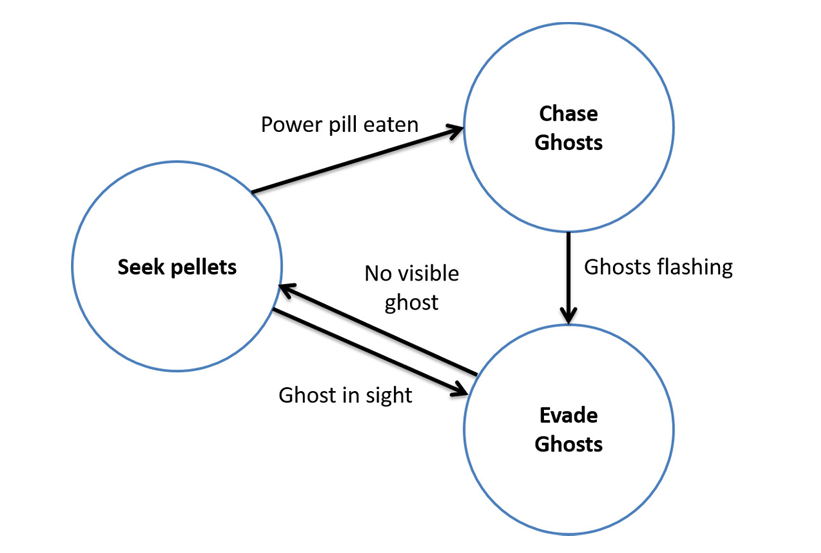
\includegraphics[width = 0.7\textwidth]{Imagenes/FMS_MsPac-man.png}
	\caption{Comportamiento jugador Pac-Man, extraído del libro de Yannakakis y Togelius (2018)}
	\label{fig:Comportamiento jugador Pac-Man}
\end{figure}

Un punto en contra de las FSMs es que son muy inflexibles y estáticas, de manera que las posibilidades de escalado de la lógica son limitadas. También son algo predecibles una vez el jugador ha estudiado los estados y transiciones de una entidad, este punto negativo puede paliarse implementado probabilidades o reglas que no estén tan claras a la hora de hacer las transiciones.

\subsection{Árboles de comportamiento}

\subsection{Goal-Oriented Action Planning}
\comp{https://github.com/crashkonijn/GOAP herramienta que podriamos analizar}\\ 
\subsection{Aprendizaje por Refuerzo (RL) o Redes Neuronales}
\section{Análisis herramientas}
\subsection{Behaviour Bricks}
\subsection{Play Maker}
\subsection{Animator}
\section{Motores de videojuegos}
\subsection{Unity}
\subsection{Unreal}
\subsection{Godot}
\subsection{GameMaker}
\subsection{Construct 3}
\section{Conclusiones}
-----------------------------------------------------\\
En el estado de la cuestión es donde aparecen gran parte de las referencias bibliográficas del trabajo. Una de las formas más cómodas de gestionar la bibliografía en {\LaTeX} es utilizando \textbf{bibtex}. Las entradas bibliográficas deben estar en un fichero con extensión \textit{.bib} (con esta plantilla se proporciona el fichero biblio.bib, donde están las entradas referenciadas más abajo). Cada entrada bibliográfica tiene una clave que permite referenciarla desde cualquier parte del texto con los siguiente comandos:

\begin{itemize}
\item Referencia bibliografica con cite: \cite{ldesc2e}
\item Referencia bibliográfica con citep: \citep{notsoshort}
\item Referencia bibliográfica con citet: \citet{latexAPrimer}
\end{itemize}

Es posible citar más de una fuente, como por ejemplo \citep{latexCompanion,LaTeXLamport,texKnuth}

Después, \LaTeX se ocupa de rellenar la sección de bibliografía con las entradas \textbf{que hayan sido citadas} (es decir, no con todas las entradas que hay en el .bib, sino sólo con aquellas que se hayan citado en alguna parte del texto).

Bibtex es un programa separado de latex, pdflatex o cualquier otra cosa que se use para compilar los .tex, de manera que para que se rellene correctamente la sección de bibliografía es necesario compilar primero el trabajo (a veces es necesario compilarlo dos veces), compilar después con bibtex, y volver a compilar otra vez el trabajo (de nuevo, puede ser necesario compilarlo dos veces). 

\chapter{Descripción del Trabajo}
\label{cap:descripcionTrabajo}

Aquí comienza la descripción del trabajo realizado. Se deben incluir tantos capítulos como sea necesario para describir de la manera más completa posible el trabajo que se ha llevado a cabo. Como muestra la figura \ref{fig:sampleImage}, está todo por hacer.

\begin{figure}[h]
	\centering
	
\includegraphics[width = 0.5\textwidth]{Imagenes/Vectorial/Todo.pdf}
	\caption{Ejemplo de imagen}
	\label{fig:sampleImage}
\end{figure}

Si te sirve de utilidad,  puedes incluir tablas para mostrar resultados, tal como se ve en la tabla \ref{tab:sampleTable}.


\begin{table}
	\centering
	\begin{tabular}{c|c|c}
		\textbf{Col 1} & \textbf{Col 2} & \textbf{Col 3} \\
		\hline\hline
		3 & 3.01 & 3.50\\
		6 & 2.12 & 4.40\\
		1 & 3.79 & 5.00\\
		2 & 4.88 & 5.30\\
		4 & 3.50 & 2.90\\
		5 & 7.40 & 4.70\\
		\hline
	\end{tabular}
	\caption{Tabla de ejemplo}
	\label{tab:sampleTable}
\end{table}

\setcounter{secnumdepth}{3} %para tener una profundidad más en las enumeraciones
\chapter{Implementaci\'on}
\label{cap:implementacion}
En el Capítulo 3 se abordó la descripción de la herramienta sin entrar en detalles de como funcionaba esta por debajo, una visión general de lo que se iba a ofrecer, como la organización de los componentes, los tipos de daño o los diferentes tipos de actuadores. En este capítulo se va a tratar en profundidad la implementación de estos componentes, hablando de cómo funcionan, cómo se pueden personalizar y como los distintos componentes interactúan entre ellos.


\section{Tecnología utilizada}
Este proyecto ha sido desarrollado íntegramente con el motor de videojuegos Unity, mencionado en el Capítulo 2 de este trabajo.
La versión escogida para desarrollar la herramientas es la 2022.3.18f1, por lo que no podemos garantizar que la herramienta funcione en versiones anteriores a la mencionada y en el caso de la versiones posteriores debería funcionar sin ningún problema a no ser que la API básica de Unity cambie en un futuro.\\
\comp{En trabajo futuro podemos poner que en caso de que se cambie la API básica necesitaría algo de mantenimiento básico.}

Unity es una herramienta muy versátil, la cúal se adapta muy bien a un gran rango de aplicaciones diferentes entre sí, desde entornos simples en dos dimensiones hasta entornos mucho más complejos en tres dimensiones, incluso en realidad virtual o realidad aumentada.
Unity surge de la idea de acercar el desarrollo de videojuegos a segmentos de la población que se podrían ver abrumados por la necesidad de entender de programación para realizar sus proyectos ya sean estos profesionales o amateurs.Este motor de videojuegos ofrece soporte para varios lenguajes de programación a través de su sistema de \textit{plugins}, de manera nativa Unity nos ofrece los lenguajes C\# y Javascript como principales lenguajes de programación de \textit{scripts}.\\

Unity no solo se usa para videojuegos, también para simuladores didácticos, cine o para modelar.
Interfaz de usuario muy gráfica, intuitiva dentro de su complejidad, y fácilmente personalizable.
Sistema de arrastrar soltar para construir escenas y/o asignar scripts.
Curva de aprendizaje no muy pronunicada gracias a su extensa documentación y la cantidad de videos y tutoriales.
Hablar de que al ser un motor de videojuegos gratuito a priori se ha creado una comunidad muy extensa de desarrolladores muy activa que suelen contestar las preguntas.\\


¿Por qué Unity?\\
1.-Por ser accesible y sencillo.\\
2.-Por ser un motor con una gran cantidad de usuarios usándolo (útil para pruebas de usuario y para conocer nuestros errores) ya que nos da ciertas garantías de que nuestra herramienta será usada y servirá para confeccionar un mínimo de proyectos.\\
3.-Sistema de arrastrar y soltar el cual facilita el uso de nuestra herramienta y la comprensión de la misma.\\
4.-Sus sistema son de mucha ayuda y muy fáciles de implementar dentro de nuestra herramienta como el motor de físicas 2D o las herramientas que tiene para ayudar al usuario a debuggear, Gizmos.\\
5.-Arquitectura por componentes, modularidad, capacidad de abstraer la implementacion de cada componente.\\

\section{Infraestructura básica}

Componentes ajenos a nuestro sistema de estados, sensors, actuators...
Life, Player Controller...



\section{Actuators}
Hablar de los actuators
\subsection{Movement}
Movement contenido a ver si sale guay
\subsubsection{AAAA}
aaaaa
\subsection{Spawner}
Spawner
\section{Sensors and emitters}
Contenido
\subsection{Sensors}
mas contenido
\subsection{Emitters}
muchisimo mas

\setcounter{secnumdepth}{3} %para tener una profundidad más en las enumeraciones
\chapter{Evaluacion Con Usuarios}
\label{cap:evaluacionConUsuarios}
En este capítulo se hará una investigación sobre las técnicas, herramientas y formas de crear inteligencias artificiales para enemigos.
Para ello vamos a comenzar haciendo un recorrido por elementos generales relacionados con la inteligencia artificial y cómo se usan en videojuegos 2D de plataformas, ya sea para crear un NPC, un enemigo o para optimizar alguna función más a bajo nivel del juego.
Se mencionarán además herramientas para conseguir los fines descritos anteriormente y se hablará de algunos motores de videojuegos que han inspirado algunos aspectos de nuestra herramienta. \\


\section{Tecnología utilizada}
Unity.
	Por que se escogió Unity
De donde salen los sprites y cosas

La Inteligencia Artificial (IA) es la capacidad que tiene un sistema o software de realizar tareas diferentes entre sí de manera autónoma aplicando reglas, algoritmos o patrones de aprendizaje automático, simulando así comportamientos propios de la inteligencia humana.
El potencial de la IA hoy día y por lo que está generando tanto furor es su capacidad de autonomía, ya que no solo sigue reglas, si no que puede llegar a tener la capacidad de tomar decisiones.\\
En el ámbito de los videojuegos, la IA se ha hecho paso a base de demostrar su gran capacidad de adaptación a contextos diversos como la adaptación a las acciones del jugador del Alien en \textit{Alien Isolation}\footnote{\url{https://www.gamedeveloper.com/design/the-perfect-organism-the-ai-of-alien-isolation}} , la manera en la que puede generar contenido procedural para juegos roguelike como \textit{Hades}\footnote{\url{https://hades.fandom.com/es/wiki/Hades_(juego)}} o, por último, entrenar una IA para que se acerque lo máximo posible al comportamiento de un humano como en la serie \textit{Forza Motosport}\footnote{\url{https://forza.fandom.com/wiki/Forza_Wiki}}, usando redes neuronales.\\


\section{Infraestructura básica}

Componentes ajenos a nuestro sistema de estados, sensors, actuators...
Life, Player Controller...


Existen muchas técnicas que se pueden abordar a la hora de modelar una IA. Para decidir cuál se ajusta mejor a un problema en concreto, es importante saber ciertos factores, como por ejemplo la complejidad esperada del comportamiento, la adaptabilidad y flexibilidad de la técnica, si queremos invertir mucho tiempo en implementar estas técnicas o queremos algo rápido de hacer y funcional o los recursos que consumen. \\
A continuación, se presentan técnicas utilizadas en videojuegos para modelar IA, las cuales hemos seleccionado porque comparten una estructura similar a la que planteamos inicialmente. Entre ellas, las maquinas finitas de estados se ajustan especialmente a nuestro enfoque y será la que utilizaremos en nuestro desarrollo.
\subsection{Maquinas de estado finitas}
Las máquinas de estado finitas (FSM), son un modelo matemático que representan un número finito de estados y una serie de transiciones entre ellos. \\

Una FSM se representa como un grafo, siendo este una representación abstracta de un conjunto de objetos, eventos, acciones o propiedades conectados entre sí, siendo estos elementos nodos (estados) que realizan acciones y comprueban la posibilidad de que haya que cambiar de nodo. 

En el ámbito de los videojuegos, las FSM son el conjunto de estados que puede tomar una entidad y la forma de llegar a estos, teniendo en cuenta que solo puede haber un estado activo en cualquier instante. \\

Como menciona \citet{FSM_Article}, el primer videojuego documentado que utilizó FSM para implementar la lógica de juego fue \textit{Spacewar!(1961)} desarrollado en el MIT por Steve Russell. Este videojuego implementaba una lógica basada en estados para manejar el comportamiento de las naves, la detección de colisiones y la física del juego. Aunque no usaba una implementación formal de máquinas de estado, sí modelaba cambios entre estados bien definidos, como el movimiento de las naves o la activación de los disparos. \\ 

\textit{Pac-Man}\footnote{\url{https://pacman.fandom.com/es/wiki/Pac-Man_Wiki:Portada}} es un videojuego que usa FSM, en el que el jugador controla un personaje amarillo en forma de círculo con una boca que se abre y cierra constantemente. Fue lanzado en 1980 por la compañía japonesa Namco (actual Bandai Namco). El objetivo de este videojuego es recorrer un laberinto e ir comiendo todos los puntos mientras evitamos cuatro fantasmas hasta que comemos una píldora de poder que nos hace invulnerable y nos da la capacidad de comer a los fantasmas. Estos huirán tras comernos la píldora.\\
La complejidad en la IA de Pac-Man es asombrosa ya que se le quiso dar profundidad al juego haciendo que cada fantasma tuviera una personalidad diferente. Para ello se implementó una máquina de estado por fantasma haciendo que la forma en la que estos interactúan con el entorno sea ligeramente diferente.
A continuación se enumerarán los fantasmas y sus formas de comportarse.
\begin{itemize}
	 \item Blinky: es el fantasma rojo y su papel es el de cazador, siendo su personalidad la más agresiva, hecho que se refleja en que es el único fantasma que comienza fuera de la casa de los fantasmas y que tras salir empieza a perseguir al jugador incansáblemente. Tiene otra característica propia, a medida que el jugador va comiendo bolitas, comienza a aumentar su velocidad.
	 \item Pinky: como su nombre indica es el fantasma de color rosa. En japonés se llama \textit Machibuse, el que tiende emboscadas. Pinky es el interceptor del juego por lo que va a tratar de cortar el camino del jugador. Es un fantasma relativamente rápido, por lo que calculará constantemente hacia donde se dirige el jugador para usar su velocidad para adelantarse y cortar el paso.
	 \item Inky: el fantasma azul es el más impredecible de todos, ya que su función es la de adoptar temporalmente la personalidad de sus otros tres compañeros.
	 \item Clyde: el fantasma naranja y el más tranquilo de todos. Suele ser el último en salir de la casa de los fantasmas y no intentará atrapar al jugador a no ser que este esté muy cerca de él. El resto del tiempo deambula por el mapa e intenta evitar al jugador.
\end{itemize}
Para ilustrar el funcionamiento del juego se usará la Figura \ref{fig:Comportamiento jugador Pac-Man} que representa una posible FSM para el jugador, lo que haría que las decisiones tomadas fueran lo más eficientes posibles en el momento.\\

\begin{figure}[t]
	\centering
	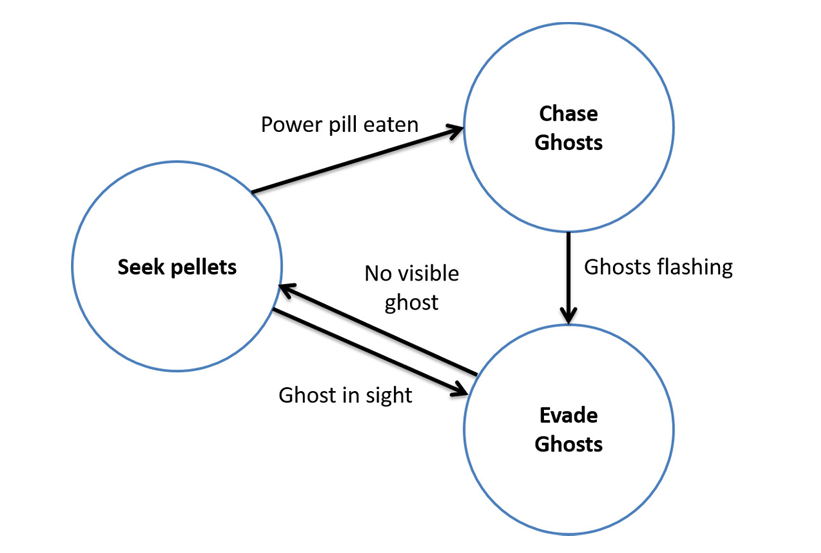
\includegraphics[width = 0.7\textwidth]{Imagenes/FMS_MsPac-man.png}
	\caption{Comportamiento jugador Pac-Man, extraído del libro de Yannakakis y Togelius (2018)}
	\label{fig:Comportamiento jugador Pac-Man}
\end{figure}

Un punto en contra de las FSMs es que son muy inflexibles y estáticas, de manera que las posibilidades de escalado de la lógica son limitadas. También son algo predecibles una vez el jugador ha estudiado los estados y transiciones de una entidad, este punto negativo puede paliarse implementado probabilidades o reglas que no estén tan claras a la hora de hacer las transiciones.

\section{Actuators}
Hablar de los actuators
\subsection{Movement}
Movement contenido a ver si sale guay
\subsubsection{AAAA}
aaaaa
\subsection{Spawner}
Spawner
\section{Sensors and emitters}
Contenido
\subsection{Sensors}
mas contenido
\subsection{Emitters}
muchisimo mas

\chapter{Conclusiones y Trabajo Futuro}
\label{cap:conclusiones}

Conclusiones del trabajo y líneas de trabajo futuro.

Antes de la entrega de actas de cada convocatoria, en el plazo que se indica en el calendario de los trabajos de fin de grado, el estudiante entregará en el Campus Virtual la versión final de la memoria en PDF.




%%%%%%%%%%%%%%%%%%%%%%%%%%%%%%%%%%%%%%%%%%%%%%%%%%%%%%%%%%%%%%%%%%%%%%%%%%%
% Si el TFG se escribe en inglés, comentar las siguientes líneas 
% porque no es necesario incluir nuevamente las Conclusiones en inglés
\begin{otherlanguage}{english}
\chapter*{Introduction}
\label{cap:introduction}
\addcontentsline{toc}{chapter}{Introduction}

\chapterquote{Human beings are not born once and for all on the day their mothers give birth to them, but rather life compels them to give birth to themselves over and over again.}{Gabriel García Márquez}

\section*{Motivation}
Over the years, video games have undergone a remarkable evolution, becoming increasingly complex. In parallel, enemies have evolved in the same way. In the specific context of two-dimensional platform games, enemies are more than mere opposition for the player—they are key to expressing the very essence of the game. Designing enemies, especially in this genre, is an ever more complex task. It is not limited to giving them a particular appearance; they must also exhibit unique behaviors and characteristics. As a result, the person entrusted with this task must possess multidisciplinary skills (art, design, programming, etc.).

In recent years, tools have emerged aimed at significantly streamlining the designers’ workflow. However, only a limited number of these focus specifically on this domain. The purpose of such tools is to ease the designer’s job, enabling them—even without programming expertise—to generate enemies with fully functional behaviors.

\section*{Objectives}
The primary objective of this work is to design and develop a framework for the Unity game engine that simplifies and accelerates the creation of enemies in 2D platform games. This framework defines a modular structure of components and behaviors based on an analysis of common enemies in this genre, with the aim of completely separating the roles of programming and design. In doing so, it enables individuals without programming knowledge to take on the role of enemy designer.

As a practical demonstration of the framework, a functional Unity tool has been developed that allows users to implement and utilize these components in a visual and intuitive way. The tool includes an easy-to-use catalog of behaviors, as well as a user manual that clearly explains each component, its installation, and usage examples.

To carry out this development, a structured work plan was followed, covering everything from the environment study and review of existing enemies to the tool’s implementation, its validation with users, and the analysis of the obtained results.

\section*{Work Plan}
This project follows the Scrum agile methodology, which creates a workflow focused on iteration and continuous improvement, ensuring efficient progress and the ability to adapt to issues as they arise. The work is divided into four main phases: research and planning, tool development, user testing, and thesis writing. Each phase is subdivided as follows:

\begin{itemize}
  \item \textbf{Research and Planning:}
    \begin{itemize}
      \item \emph{Problem Study:} In this initial phase, a state-of-the-art review will be conducted, focusing on the role of enemies in video games, their impact on gameplay, and the various techniques used in their design and behavior.
      \item \emph{Tool Selection and Analysis:} This phase involves a comparative analysis of different techniques and game engines, evaluating their advantages and disadvantages, as well as studying their architectures and workflows.
      \item \emph{Enemy Behavior Study:} This study will provide a solid foundation for the tool’s design by identifying common patterns in the behaviors of different enemies.
    \end{itemize}

  \item \textbf{Tool Development:}
    \begin{itemize}
      \item \emph{Design:} Define the proposed tool’s architecture, detailing the techniques employed, operation schemes, and organization of its main elements.
      \item \emph{Implementation of Core Features:} Develop the core functionalities for basic movements, including integration with sensors and actuators to enable interaction between them.
      \item \emph{Visual Aid Implementation:} Create visual aids intended to serve as references for designers, including graphical elements that facilitate understanding of behaviors.
      \item \emph{Testing and Debugging:} Carry out iterative tests to ensure the tool functions correctly, fixing any errors identified during implementation.
    \end{itemize}

  \item \textbf{User Testing:}
    \begin{itemize}
      \item Conduct tests with users who have not previously used the tool, following the plan detailed in Section~\ref{cap:evaluacionConUsuarios}. These tests will focus on uncovering potential issues with core features, validating functionality, and evaluating usability and clarity.
    \end{itemize}

  \item \textbf{Thesis Writing:}
    \begin{itemize}
      \item \emph{Initial Drafting:} Produce the initial draft covering all points specified in the thesis outline.
      \item \emph{Review and Revision:} Perform thorough reviews of the document and implement necessary corrections.
      \item \emph{Conclusions and Future Work:} After completing development and user testing, write the conclusions based on the results and outline possible future directions.
    \end{itemize}
\end{itemize}

\begin{figure}[h!]
  \centering
  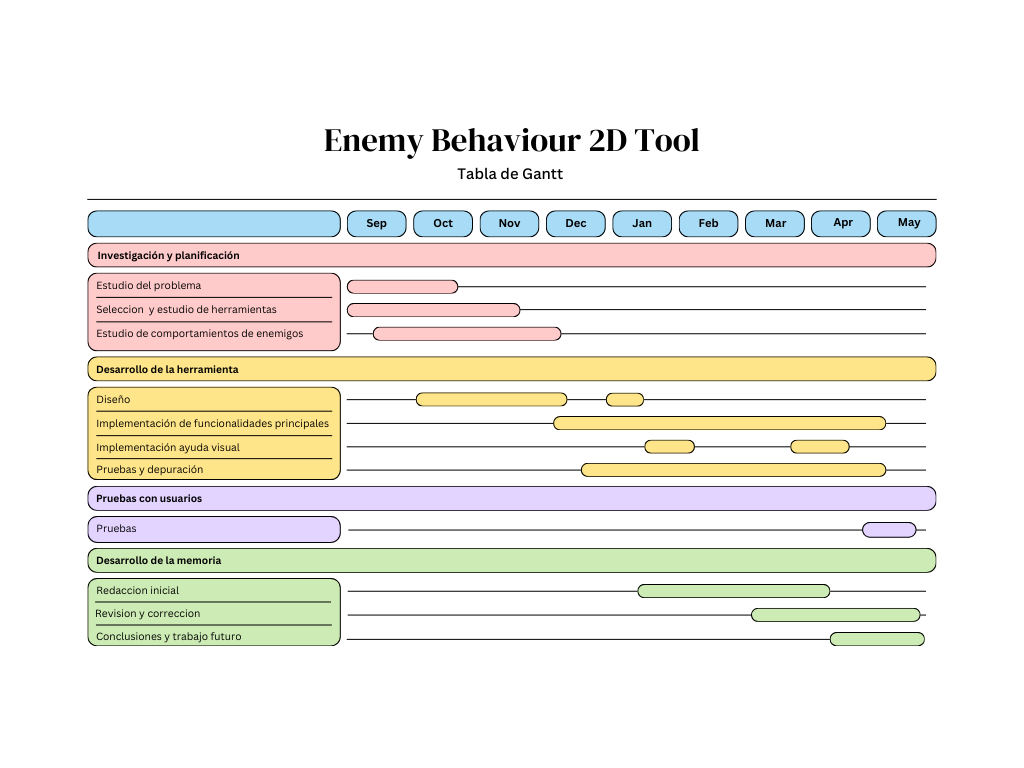
\includegraphics[height=12cm]{Imagenes/GanttChart}
  \caption{Gantt chart for the planning of the Enemy Behaviour 2D tool development}
  \label{fig:GanttEnemyBehaviour2D}
\end{figure}

\chapter*{Conclusions and Future Work}
\label{cap:conclusions}
\addcontentsline{toc}{chapter}{Conclusions and Future Work}
\section*{Final Conclusions}
This tool has been consistently focused on the design of 2D enemies. The proposal arises as a response to the need to provide designers with a practical and accessible solution that allows them to configure complex behaviors without requiring advanced programming knowledge.\\
Through an architecture based on finite state machines, and complemented by a set of sensors, actuators, and emitters, a flexible, accessible, and scalable solution has been achieved.\\
During development, essential aspects such as movement, damage control, entity generation, collision handling, and animation linking have been covered. In addition, a manual aimed at non-technical users has been included, which reinforces the accessibility purpose of the tool.


\section*{Future Work}

Looking towards future iterations, several areas of expansion have been identified that will allow the tool to have more functionalities and therefore versatility:\\
\begin{itemize}
  \item \textbf{Evolutionary Maintenance:} Periodic reviews will be necessary to ensure compatibility with future versions of the Unity engine, especially in the face of possible modifications to its base API.
  \item \textbf{Implementation of Sound Sensors:} Incorporating a sound sensor capable of detecting auditory stimuli was proposed, which would expand the interaction possibilities of enemies within the game.
  \item \textbf{Sound Emitters:} Complementary to acoustic sensors, these components would allow the emission of auditory signals that trigger behaviors in other nearby entities, enabling new game dynamics.
  \item \textbf{Steering and Avoidance Behaviors:} Integrating evasion techniques and conscious environment navigation is proposed, which would give enemies the ability to avoid obstacles and move more realistically.
  \item \textbf{Memory of Previous Interactions:} An advanced functionality would consist of allowing enemies to store information about past player actions, adapting their responses based on recognized patterns.
\item \textbf{Coordination Between Enemies:} Another line of improvement is to allow communication and cooperation between multiple enemies, generating collective behavior patterns, such as group chases or synchronized attacks.
 \item \textbf{Development of an External Graphical Interface:} In the long term, it is suggested to design an independent visual interface that facilitates the selection and configuration of components through a specific window, thus optimizing the user experience.
\end{itemize}

These lines of work reflect the potential of the system as an active tool within the 2D video game development workflow. The modular structure and the orientation towards scalability will allow these improvements to be incorporated progressively, guaranteeing its usefulness in real projects for the design of complex enemies.
\end{otherlanguage}
%%%%%%%%%%%%%%%%%%%%%%%%%%%%%%%%%%%%%%%%%%%%%%%%%%%%%%%%%%%%%%%%%%%%%%%%%%%

\chapter*{Contribuciones Personales}
\label{cap:contribucionesPersonales}
\addcontentsline{toc}{chapter}{Contribuciones Personales}

\section*{Contribuciones de Francisco Miguel Galván Muñoz}
\subsection*{Antecedentes}
Antes de comenzar este proyecto, ya tenía una base sólida sobre Máquinas de Estados gracias a asignaturas como \textit{Fundamentos de Computadores} e \textit{Inteligencia Artificial}, donde implementamos por primera vez una en Unity. En esa práctica, la arquitectura propuesta resultó poco escalable y compleja, especialmente para modelar comportamientos básicos como patrullar, perseguir o atacar, lo que motivó mi interés por buscar soluciones más eficientes.\\

Aunque siempre me había interesado el diseño de enemigos, no lo había explorado teóricamente hasta este proyecto. Durante su desarrollo, investigamos patrones comunes en enemigos de videojuegos 2D, lo que nos permitió identificar comportamientos reutilizables y orientar nuestra herramienta hacia una arquitectura modular y accesible para desarrolladores.\\
 
\subsection*{Aportación}
\subsubsection*{Investigación}
Cuando comenzamos con la etapa de investigación, a mediados de septiembre, tanto Cristina como yo seleccionamos varios videojuegos con el objetivo de analizar el comportamiento de sus enemigos más representativos. En mi caso, elegí \textit{Blasphemous} y adopté una dinámica basada en la observación directa: mientras jugaba, capturaba imágenes cada vez que aparecía un enemigo nuevo y realizaba un análisis detallado de su comportamiento. Esta dinámica la mantuve durante las primeras tres horas de juego, lo cual me permitió identificar paralelismos entre distintos tipos de enemigos, especialmente en lo referente a la forma en que se activaban las transiciones entre estados y cómo variaban sus comportamientos en función del estado en el que se encontraban.\\

Paralelamente a esta labor práctica, llevé a cabo una investigación teórica consultando artículos académicos (\textit{papers}) y conferencias de la GDC (Game Developers Conference), con el fin de comprender cómo se aborda el diseño de enemigos a nivel profesional. Esta información fue de gran utilidad para dar forma a los fundamentos de nuestra herramienta.\\

Una vez finalizada la fase de recopilación de información por ambas partes, celebramos varias reuniones para poner en común los hallazgos, identificar similitudes entre nuestros análisis y definir una base conceptual común. Gracias a este trabajo colaborativo, pudimos orientar adecuadamente la arquitectura de la herramienta, y comenzamos con el diseño e implementación de los primeros sensores y actuadores que formarían parte del sistema.\\

\subsubsection*{Confección de la herramienta}

Durante las primeras fases del desarrollo de la herramienta, decidimos trabajar conjuntamente para establecer una estructura base que fuera modular y con una lógica coherente. A partir de ahí, me encargué del desarrollo del sistema de gestión de daño, así como de varios actuadores, como el \textit{Move To A Point Actuator} y el \textit{Directional Actuator}. \\

También me responsabilicé de implementar la lógica necesaria para asegurar que los parámetros requeridos por cada componente de la herramienta fueran los adecuados en cada caso. Esta lógica se encuentra contenida en un \textit{script} editor asociado a cada componente, lo que permite una configuración dinámica y contextual según el tipo de actuador o sensor seleccionado.\\

\subsubsection*{Parte de la memoria}

En cuanto a la redacción de la memoria, me encargué del resumen inicial del documento y del capítulo correspondiente al estado de la cuestión. Dentro del apartado de implementación, redacté todos los subapartados excepto el 4.3 y el 4.5. Asimismo, en la sección de evaluación con usuarios, fui responsable de describir el rol del investigador, la metodología de observación y el proceso de puesta en común de los resultados obtenidos.\\

\subsubsection*{Manual}
Mi participación en la elaboración del manual se centró en la corrección de errores, la traducción del contenido del español al inglés y la integración del glosario, asegurando que se explicaran adecuadamente los términos clave utilizados en la herramienta.\\

\section*{Contribuciones de Cristina Mora Velasco}
\subsubsection*{Investigación}
\subsubsection*{Confección de la herramienta}
\subsubsection*{Parte de la memoria}
\subsubsection*{Manual}



%
% Bibliografía
%
% Si el TFM se escribe en inglés, editar TeXiS/TeXiS_bib para cambiar el
% estilo de las referencias
%---------------------------------------------------------------------
%
%                      configBibliografia.tex
%
%---------------------------------------------------------------------
%
% bibliografia.tex
% Copyright 2009 Marco Antonio Gomez-Martin, Pedro Pablo Gomez-Martin
%
% This file belongs to the TeXiS manual, a LaTeX template for writting
% Thesis and other documents. The complete last TeXiS package can
% be obtained from http://gaia.fdi.ucm.es/projects/texis/
%
% Although the TeXiS template itself is distributed under the 
% conditions of the LaTeX Project Public License
% (http://www.latex-project.org/lppl.txt), the manual content
% uses the CC-BY-SA license that stays that you are free:
%
%    - to share & to copy, distribute and transmit the work
%    - to remix and to adapt the work
%
% under the following conditions:
%
%    - Attribution: you must attribute the work in the manner
%      specified by the author or licensor (but not in any way that
%      suggests that they endorse you or your use of the work).
%    - Share Alike: if you alter, transform, or build upon this
%      work, you may distribute the resulting work only under the
%      same, similar or a compatible license.
%
% The complete license is available in
% http://creativecommons.org/licenses/by-sa/3.0/legalcode
%
%---------------------------------------------------------------------
%
% Fichero  que  configura  los  parámetros  de  la  generación  de  la
% bibliografía.  Existen dos  parámetros configurables:  los ficheros
% .bib que se utilizan y la frase célebre que aparece justo antes de la
% primera referencia.
%
%---------------------------------------------------------------------


%%%%%%%%%%%%%%%%%%%%%%%%%%%%%%%%%%%%%%%%%%%%%%%%%%%%%%%%%%%%%%%%%%%%%%
% Definición de los ficheros .bib utilizados:
% \setBibFiles{<lista ficheros sin extension, separados por comas>}
% Nota:
% Es IMPORTANTE que los ficheros estén en la misma línea que
% el comando \setBibFiles. Si se desea utilizar varias líneas,
% terminarlas con una apertura de comentario.
%%%%%%%%%%%%%%%%%%%%%%%%%%%%%%%%%%%%%%%%%%%%%%%%%%%%%%%%%%%%%%%%%%%%%%
\setBibFiles{%
biblio%
}

%%%%%%%%%%%%%%%%%%%%%%%%%%%%%%%%%%%%%%%%%%%%%%%%%%%%%%%%%%%%%%%%%%%%%%
% Definición de la frase célebre para el capítulo de la
% bibliografía. Dentro normalmente se querrá hacer uso del entorno
% \begin{FraseCelebre}, que contendrá a su vez otros dos entornos,
% un \begin{Frase} y un \begin{Fuente}.
%
% Nota:
% Si no se quiere cita, se puede eliminar su definición (en la
% macro setCitaBibliografia{} ).
%%%%%%%%%%%%%%%%%%%%%%%%%%%%%%%%%%%%%%%%%%%%%%%%%%%%%%%%%%%%%%%%%%%%%%
\setCitaBibliografia{
\begin{FraseCelebre}
\begin{Frase}
Jugamos no solo para escapar de la realidad, sino para encontrar una versión más intensa de ella.
\end{Frase}
\begin{Fuente}
 Jane McGonigal
\end{Fuente}
\end{FraseCelebre}
}

%%
%% Creamos la bibliografia
%%
\makeBib

% Variable local para emacs, para  que encuentre el fichero maestro de
% compilación y funcionen mejor algunas teclas rápidas de AucTeX

%%%
%%% Local Variables:
%%% mode: latex
%%% TeX-master: "../Tesis.tex"
%%% End:



% Apéndices
\appendix
\chapter{Título del Apéndice A}
\label{Appendix:Key1}

Los apéndices son secciones al final del documento en las que se agrega texto con el objetivo de ampliar los contenidos del documento principal.
\chapter{Título del Apéndice B}
\label{Appendix:Key2}

Se pueden añadir los apéndices que se consideren oportunos.
%\include{Apendices/appendixC}
%\include{...}
%\include{...}
%\include{...}
\backmatter



%
% Índice de palabras
%

% Sólo  la   generamos  si  está   declarada  \generaindice.  Consulta
% TeXiS.sty para más información.

% En realidad, el soporte para la generación de índices de palabras
% en TeXiS no está documentada en el manual, porque no ha sido usada
% "en producción". Por tanto, el fichero que genera el índice
% *no* se incluye aquí (está comentado). Consulta la documentación
% en TeXiS_pream.tex para más información.
\ifx\generaindice\undefined
\else
%%---------------------------------------------------------------------
%
%                        TeXiS_indice.tex
%
%---------------------------------------------------------------------
%
% TeXiS_indice.tex
% Copyright 2009 Marco Antonio Gomez-Martin, Pedro Pablo Gomez-Martin
%
% This file belongs to TeXiS, a LaTeX template for writting
% Thesis and other documents. The complete last TeXiS package can
% be obtained from http://gaia.fdi.ucm.es/projects/texis/
%
% This work may be distributed and/or modified under the
% conditions of the LaTeX Project Public License, either version 1.3
% of this license or (at your option) any later version.
% The latest version of this license is in
%   http://www.latex-project.org/lppl.txt
% and version 1.3 or later is part of all distributions of LaTeX
% version 2005/12/01 or later.
%
% This work has the LPPL maintenance status `maintained'.
% 
% The Current Maintainers of this work are Marco Antonio Gomez-Martin
% and Pedro Pablo Gomez-Martin
%
%---------------------------------------------------------------------
%
% Contiene  los  comandos  para  generar  el índice  de  palabras  del
% documento.
%
%---------------------------------------------------------------------
%
% NOTA IMPORTANTE: el  soporte en TeXiS para el  índice de palabras es
% embrionario, y  de hecho  ni siquiera se  describe en el  manual. Se
% proporciona  una infraestructura  básica (sin  terminar)  para ello,
% pero  no ha  sido usada  "en producción".  De hecho,  a pesar  de la
% existencia de  este fichero, *no* se incluye  en Tesis.tex. Consulta
% la documentación en TeXiS_pream.tex para más información.
%
%---------------------------------------------------------------------


% Si se  va a generar  la tabla de  contenidos (el índice  habitual) y
% también vamos a  generar el índice de palabras  (ambas decisiones se
% toman en  función de  la definición  o no de  un par  de constantes,
% puedes consultar modo.tex para más información), entonces metemos en
% la tabla de contenidos una  entrada para marcar la página donde está
% el índice de palabras.

\ifx\generatoc\undefined
\else
   \addcontentsline{toc}{chapter}{\indexname}
\fi


% Generamos el índice
\printindex

% Variable local para emacs, para  que encuentre el fichero maestro de
% compilación y funcionen mejor algunas teclas rápidas de AucTeX

%%%
%%% Local Variables:
%%% mode: latex
%%% TeX-master: "./tesis.tex"
%%% End:

\fi

%
% Lista de acrónimos
%

% Sólo  lo  FSM_ArticleFSM_Article  si  está declarada  \generaacronimos.  Consulta
% TeXiS.sty para más información.


\ifx\generaacronimos\undefined
\else
%---------------------------------------------------------------------
%
%                        TeXiS_acron.tex
%
%---------------------------------------------------------------------
%
% TeXiS_acron.tex
% Copyright 2009 Marco Antonio Gomez-Martin, Pedro Pablo Gomez-Martin
%
% This file belongs to TeXiS, a LaTeX template for writting
% Thesis and other documents. The complete last TeXiS package can
% be obtained from http://gaia.fdi.ucm.es/projects/texis/
%
% This work may be distributed and/or modified under the
% conditions of the LaTeX Project Public License, either version 1.3
% of this license or (at your option) any later version.
% The latest version of this license is in
%   http://www.latex-project.org/lppl.txt
% and version 1.3 or later is part of all distributions of LaTeX
% version 2005/12/01 or later.
%
% This work has the LPPL maintenance status `maintained'.
% 
% The Current Maintainers of this work are Marco Antonio Gomez-Martin
% and Pedro Pablo Gomez-Martin
%
%---------------------------------------------------------------------
%
% Contiene  los  comandos  para  generar  el listado de acrónimos
% documento.
%
%---------------------------------------------------------------------
%
% NOTA IMPORTANTE:  para que la  generación de acrónimos  funcione, al
% menos  debe  existir  un  acrónimo   en  el  documento.  Si  no,  la
% compilación  del   fichero  LaTeX  falla  con   un  error  "extraño"
% (indicando  que  quizá  falte  un \item).   Consulta  el  comentario
% referente al paquete glosstex en TeXiS_pream.tex.
%
%---------------------------------------------------------------------


% Redefinimos a español  el título de la lista  de acrónimos (Babel no
% lo hace por nosotros esta vez)

\def\listacronymname{Lista de acrónimos}

% Para el glosario:
% \def\glosarryname{Glosario}

% Si se  va a generar  la tabla de  contenidos (el índice  habitual) y
% también vamos a  generar la lista de acrónimos  (ambas decisiones se
% toman en  función de  la definición  o no de  un par  de constantes,
% puedes consultar config.tex  para más información), entonces metemos
% en la  tabla de contenidos una  entrada para marcar  la página donde
% está el índice de palabras.

\ifx\generatoc\undefined
\else
   \addcontentsline{toc}{chapter}{\listacronymname}
\fi


% Generamos la lista de acrónimos (en realidad el índice asociado a la
% lista "acr" de GlossTeX)

\printglosstex(acr)

% Variable local para emacs, para  que encuentre el fichero maestro de
% compilación y funcionen mejor algunas teclas rápidas de AucTeX

%%%
%%% Local Variables:
%%% mode: latex
%%% TeX-master: "../Tesis.tex"
%%% End:

\fi

%
% Final
%
%---------------------------------------------------------------------
%
%                      fin.tex
%
%---------------------------------------------------------------------
%
% fin.tex
% Copyright 2009 Marco Antonio Gomez-Martin, Pedro Pablo Gomez-Martin
%
% This file belongs to the TeXiS manual, a LaTeX template for writting
% Thesis and other documents. The complete last TeXiS package can
% be obtained from http://gaia.fdi.ucm.es/projects/texis/
%
% Although the TeXiS template itself is distributed under the 
% conditions of the LaTeX Project Public License
% (http://www.latex-project.org/lppl.txt), the manual content
% uses the CC-BY-SA license that stays that you are free:
%
%    - to share & to copy, distribute and transmit the work
%    - to remix and to adapt the work
%
% under the following conditions:
%
%    - Attribution: you must attribute the work in the manner
%      specified by the author or licensor (but not in any way that
%      suggests that they endorse you or your use of the work).
%    - Share Alike: if you alter, transform, or build upon this
%      work, you may distribute the resulting work only under the
%      same, similar or a compatible license.
%
% The complete license is available in
% http://creativecommons.org/licenses/by-sa/3.0/legalcode
%
%---------------------------------------------------------------------
%
% Contiene la última página
%
%---------------------------------------------------------------------


% Ponemos el marcador en el PDF
\ifpdf
   \pdfbookmark{Fin}{fin}
\fi

\thispagestyle{empty}\mbox{}

Este texto se puede encontrar en el fichero Cascaras/fin.tex. Si deseas eliminarlo, basta con comentar la línea correspondiente al final del fichero TFGTeXiS.tex.

\vspace*{4cm}

\small

\hfill \emph{--¿Qué te parece desto, Sancho? -- Dijo Don Quijote --}

\hfill \emph{Bien podrán los encantadores quitarme la ventura,}

\hfill \emph{pero el esfuerzo y el ánimo, será imposible.}

\hfill 

\hfill \emph{Segunda parte del Ingenioso Caballero} 

\hfill \emph{Don Quijote de la Mancha}

\hfill \emph{Miguel de Cervantes}

\vfill%space*{4cm}

\hfill \emph{--Buena está -- dijo Sancho --; fírmela vuestra merced.}

\hfill \emph{--No es menester firmarla -- dijo Don Quijote--,}

\hfill \emph{sino solamente poner mi rúbrica.}

\hfill 

\hfill \emph{Primera parte del Ingenioso Caballero} 

\hfill \emph{Don Quijote de la Mancha}

\hfill \emph{Miguel de Cervantes}


\newpage
\thispagestyle{empty}\mbox{}

\newpage

% Variable local para emacs, para  que encuentre el fichero maestro de
% compilación y funcionen mejor algunas teclas rápidas de AucTeX

%%%
%%% Local Variables:
%%% mode: latex
%%% TeX-master: "../Tesis.tex"
%%% End:

%\end{otherlanguage}
\end{document}
